\section{Stochastic Networks}
\label{sec:stochastic}

The VOTCA package contains the functionality of generating large, amorphous charge transport networks ($\sim10^6$ molecules). This is done with a combined coarse-grained and stochastic approach. VOTCA::CSG is used to generate a coarse-grained morphology. The stochastic modeling of VOTCA::CTP allows to make a charge transfer network out of this morphology by reproducing the neighbor list (connectivity), transfer integrals, correlated site energies. An overview is given in Figure \ref{fig:overview_stochastic}.

Througout this section we will use two state files. One is the state file \sqlstateref of the smaller reference system that can be generated as explained in the previous sections. The second one is the state file \sqlstatecg of the coarse-grained system, or the stochastic network, that can be parametrized as explained in this section.


When using the stochastic functionalities, please cite the corresponding work:

\begin{enumerate}
\item{B. Baumeier, O. Stenzel, C. Poelking, D. Andrienko, and V. Schmidt: Stochastic modeling of molecular charge transport networks. Phys. Rev. B 86, 184202 (2012)}
\item{P. Kordt and D. Andrienko: Modeling of Spatially Correlated Energetic Disorder in Organic Semiconductors. Journal of Chemical Theory and Computation 12, 36--40 (2016)}
\item{P. Kordt, J. J. M. van der Holst, M. Al Helwi, W. Kowalsky, F. May, A. Badinski, C. Lennartz, and D. Andrienko: Modeling of Organic Light Emitting Diodes: From Molecular to Device Properties. Advanced Functional Materials 25, 1955--1971 (2015)}
\end{enumerate}




\begin{figure*}[h]

\includegraphics[width=0.7\textwidth]{fig/stochastic/overview_stochastic}
\caption{Stochastic Model in VOTCA. Overview of the different steps for generating stochastic charge transport networks in VOTCA. The Molecular Dynamics software GROMACS allows to analyze the radial distribution function of a morphology, which is then used by VOTCA::CSG to generate a coarse-grained potential that reproduces this distribution function. This potential can then be used for coarse-grained simulations in GROMCAS. For calculating rates in the coarse-grained morpholgy, first the relavant parameters are extracted (panalyze, eanalyze, ianalyze) from the reference morphology and and then reproduced in the coarsed-coarse grained morphology (neighborlist, eimport, iimport). With all these at hand, the rates calculator can be used in the coarse-grained morphology.}
\label{fig:overview_stochastic}
\end{figure*}

\subsection{Coarse-grained morphology}
The first step is to generate a coarse-grained morphology. In this example, it is done by mapping a DPBIC molecule (which consists of 103 atoms) to a single point, its center of mass and by using the iterative Boltzmann inversion (IBI) method. Starting point is a smaller reference morphology, generated with GROMACS. Using the command

\texttt{g\_rdf -f traj.xtc -s topol.tpr}

you can extract the radial distribution function $g(r)$ of your reference topolgy, outputted into the file rdf.xvg. This file, together with table.xvg,grompp.mdp, topol.top, index.ndx and confout.gro form your reference data.

For VOTCA::CSG you need a \textbf{setting.xml} file:

\lstset{language=XML2}
\begin{lstlisting}
<cg>
 <!-- example for a non-bonded interaction entry -->
 <non-bonded>
  <!-- name of the interaction -->
  <name>IR-IR</name>
  <!-- types involved in this interaction -->
  <type1>IR</type1>
  <type2>IR</type2>
  <!-- dimension + grid spacing of tables for calculations -->
  <min>0.5</min>
  <max>5.0</max>
  <step>0.01</step>
  <inverse>
   <!-- target distribution (rdf), just give gromacs rdf.xvg -->
   <target>rdf.xvg</target>
   <!-- update cycles -->
   <do_potential>1</do_potential>
   <!-- additional post processing of dU before added to potential -->
   <post_update>scale smooth</post_update>
   <post_update_options>
          <scale>0.5</scale> <!--Scale the potential before updating it -->
   	<smooth>
        	<iterations>2</iterations>
   	</smooth>
   </post_update_options>
   <!-- additional post processing of U after dU added to potential -->
   <post_add></post_add>
   <!-- name of the table for gromacs run -->
   <gromacs>
    <table>table_IR_IR.xvg</table>
   </gromacs>
  </inverse>
 </non-bonded>
   
 <!-- general options for inverse script -->
 <inverse>
  <!-- 300*0.00831451 gromacs units -->
  <kBT>2.49435300</kBT>
  <initial_configuration>maindir</initial_configuration>
  <!-- use gromacs as simulation program -->
  <program>gromacs</program>
  <!-- gromacs specific options -->
  <gromacs>
     <!-- trash so many frames at the beginning -->
     <equi_time>500</equi_time>
     <!-- grid for table*.xvg !-->
     <table_bins>0.001</table_bins>
     <!-- cut the potential at this value (gromacs bug) -->
     <pot_max>1000000</pot_max>
     <!-- extend the tables to this value -->
     <table_end>6.0</table_end>
  </gromacs>
  <!-- these files are copied for each new run -->
  <filelist>grompp.mdp topol.top index.ndx table.xvg</filelist>
  <!-- do so many iterations -->
  <iterations_max>500</iterations_max>
  <!-- Try to clean a bit -->
  <cleanlist>traj.xtc</cleanlist>
  <!-- ibm: inverse boltzmann imc: inverse monte carlo -->
  <method>ibi</method>
  <!-- write log to this file -->
  <log_file>inverse.log</log_file>
  <!-- write restart step to this file -->
  <restart_file>restart_points.log</restart_file>
  <!-- imc specific stuff -->
 </inverse>
</cg>
\end{lstlisting}

You run IBI using the command

\texttt{csg\_inverse --options settings.xml}

IBI intents to find a pontential $U(r)$ that reproduces your radial distribution function. It is stored in the file \textbf{table\_IR\_IR.xvg} in our example.

With the interaction potential at hand, a large topology can be generated using molecular dynamics simulations for the coarse grained model. Starting point is a box with equally distributed points, with each point representing one molecule and with the number of points chosen such that the density of the reference system is reproduced. A small python script can generate the conf.gro to start from, here shown to obtain a $50\times50\times120~{\rm nm}^3$ starting morphology.

\lstset{language=Python}
\begin{lstlisting}

from pylab import *
import numpy as np

lenX      =  50
lenY      =  50 
lenZ      =  120 
originalV = 4704.339 
originalN = 4000
spacing   = (originalV/originalN)**(1./3.) 

molecule  = "DPBIC"
resname   = "IRI"
atomname  = "IR"

newV = lenX*lenY*lenZ
newN = int(newV/originalV*originalN)

nX   = int(lenX/spacing)+1
nY   = int(lenY/spacing)+1
nZ   = int(lenZ/spacing)+1

print "max. molecules in X direction:  "+str(nX)
print "max. molecules in Y direction:  "+str(nY)
print "max. molecules in Z direction:  "+str(nZ)
print "total number of molecules: "+str(newN)

file = open("box.gro", "w")
file.write(molecule+"\n")
file.write(str(newN)+"\n")

atomnumber = 1
for iX in range(nX):
    for iY in range(nY):
        for iZ in range(nZ):
            if(atomnumber > newN):
                break
            posX = spacing*iX
            posY = spacing*iY
            posZ = spacing*iZ
            print >> file, "%5d%-5s%5s%5d%8.3f%8.3f%8.3f%8.4f%8.4f%8.4f" % \
            (1,resname,atomname,1,posX,posY,posZ,0,0,0)
            atomnumber += 1


file.write("  "+str(lenX)+"  "+str(lenY)+"  "+str(lenZ))
file.close()

print "Note: for some obscure reason VMD will not be able to read this file\
properly unless you open it once in vi and save it."


\end{lstlisting}

Open the box.gro in vi and save it (\texttt{:wq}), afterwards you can have a look at it in VDM. Run your MD simulations using the \texttt{mdrun} command. In the end you can compare the radial distribution functions of your reference and coarse-grained system, as shown in figure \ref{fig:stochastic}(a) as an example.

\subsection{Charge transport network}

\begin{figure*}[ht]
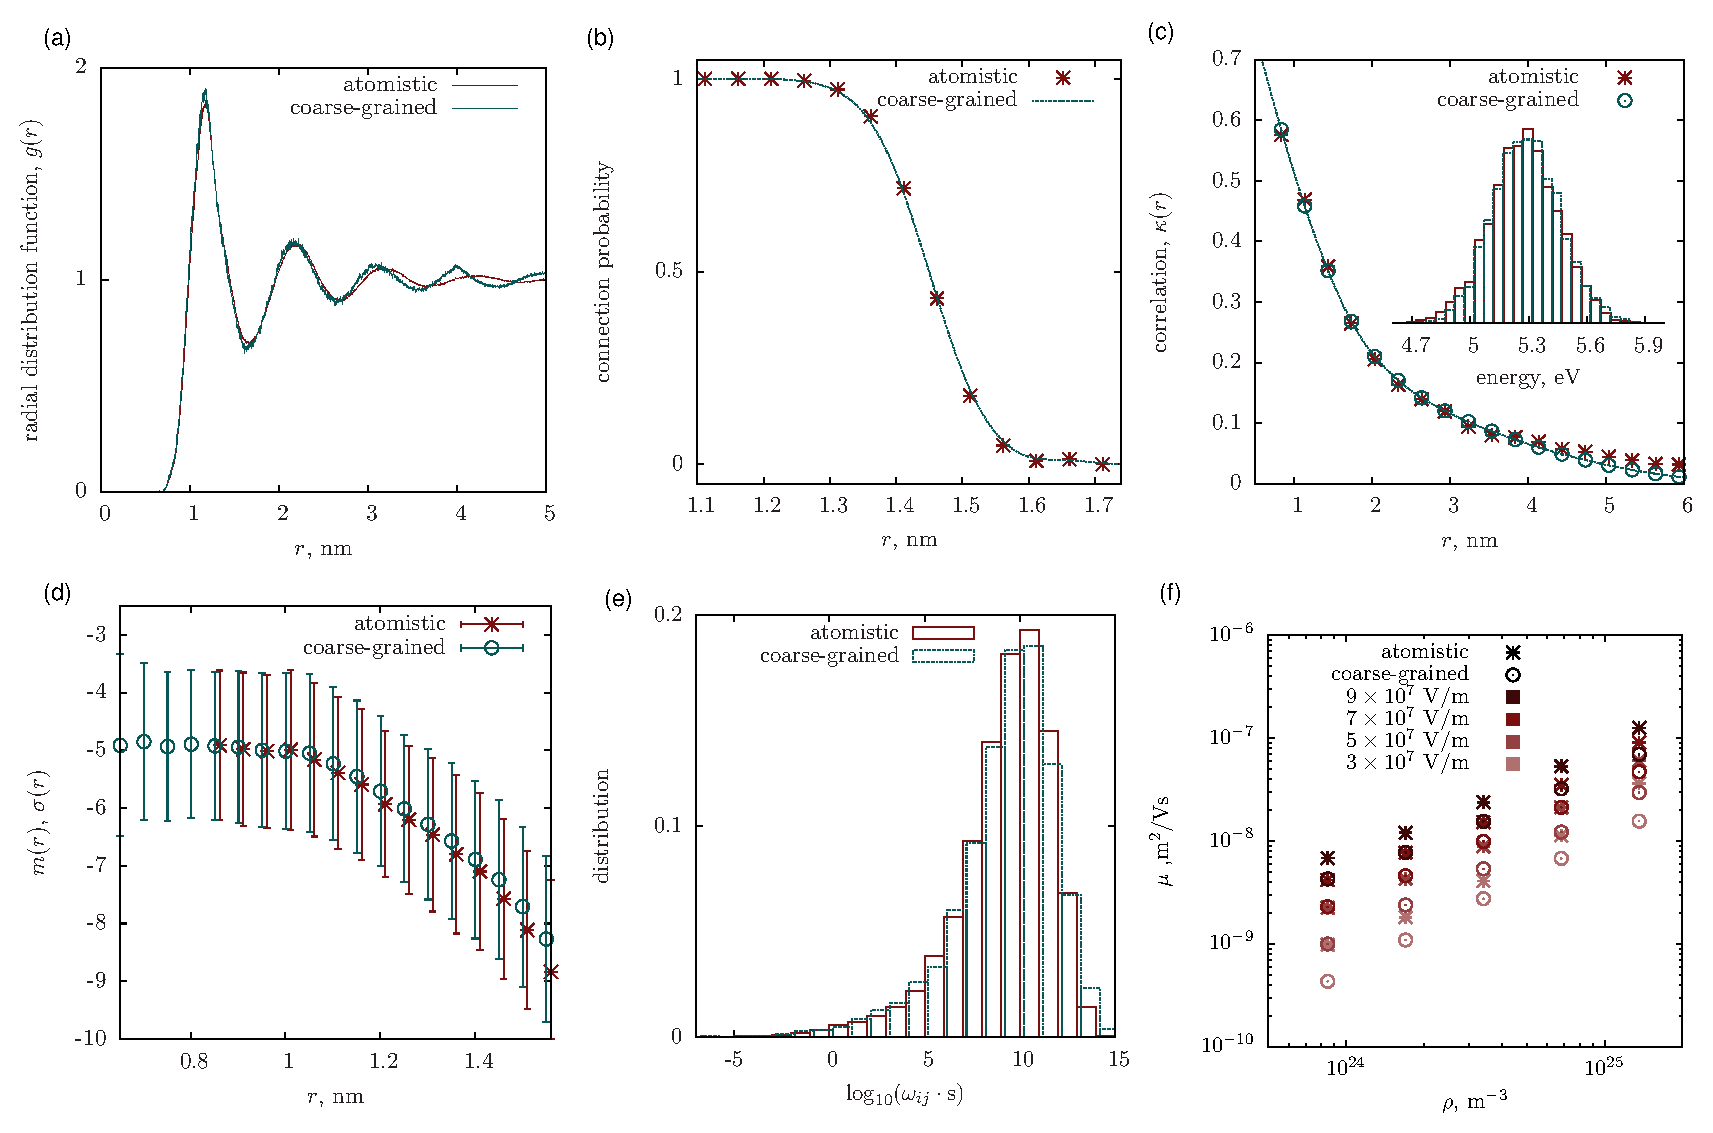
\includegraphics[width=1.0\textwidth]{fig/stochastic/stochastic}
\caption{ Comparison of the atomistic ($\unit[17\times17\times17]{nm^3}$) and coarse-grained ($\unit[50\times 50\times120]{nm^3}$) models. (a) Radial distribution function, $g(r)$. (b) Probability of two sites to be connected (added to the neighbor list) as a function of their separation. (c) Spatial site energy autocorrelation function, $\kappa(r)$; Inset:  Site energy distribution. (d) Mean $m$ and width $\sigma$ of a distribution of the logarithm of electronic couplings, $\log_{10}(\unit[J^2/]{eV^2})$, for molecules at a fixed separation $r$. (e) Rate distributions. (f) Mobility as a function of hole density, plotted for four different electric fields.}
\label{fig:stochastic}
\end{figure*}

To generate a charge transport network you first need a reference system with neighbor list, site energies and transfer integrals calculated and stored in a \textbf{state.sql} state file. The procedure for all these three properties is always the same: first analyze the reference data, and second import the analyzation files and reproduce the properties.




\subsubsection{Neighbor list}

In the atomistic reference system molecules are connected if their two closest segments are below a certain cut-off radius. This finer picture of segments does not exist in the coarse-grained system, where each molecule is represented by a point. To mimick the neighbor list, the probability of two molecules to be connected is analyzed as a function of their center-of-mass distance. This can be done by using the \emph{panalyze} calculator

\votcacommand{Analyze the pair connectivity (neighborlist) in the reference system}{\cmdpanalyze}

with the options defined as follows:
\\

\textbf{options\_analyze.xml}

\lstset{language=XML2}
\begin{lstlisting}
<options>
        <panalyze>
                <resolution_space>0.05</resolution_space>
        </panalyze>
</options>
\end{lstlisting}

The only parameter needed is the spacial resolution, i.e., the bin size for calculating the probabilities. The \emph{panalyze} calculator outputs a file \textbf{panalyze.distanceprobability.out} with the respective probabilities.
Now this file has to be imported into the coarse-grained state file

\votcacommand{Import the reference pair connectivity (neighborlist) and reproduce it in stochastic network}{\cmdnblst}

using the following options:
\\

\textbf{options\_import.xml}

\lstset{language=XML2}
\begin{lstlisting}
<options>
	<neighborlist>
                <probabilityfile>panalyze.distanceprobability.out</probabilityfile>
	</neighborlist>
</options>
\end{lstlisting}

For testing purposes, you can run the \emph{panalyze} calculator on your coarse-grained state file and compare the probability function to the reference. An example is shown in figure \ref{fig:stochastic}(b). You can also also look at the file \textbf{panalyze.distanceprobability.out} for both state files, which has the distribution of coordination numbers (number of neighbors) and its average in.

\subsubsection{Site energies}

Site energies in amorphous organic semiconductors are roughly Gaussian distributed, with the width of the Gaussian, $\sigma$, called the energetic disorder. However, there are correlations between sites if they are close enough to each other. The aim in this section is therefore to reproduce the correlated energetic landscape.
The first step is to get a spatial correlation function as well as the mean energy and the energetic disorder from your reference state file:
\\
\votcacommand{Analyze the energy distribution and correlation in the reference system}{\cmdeanast}

with the following options:
\\

\textbf{options\_analyze.xml}

\lstset{language=XML2}
\begin{lstlisting}
<options>
        <eanalyze>
                <resolution_sites>0.05</resolution_sites>
                <resolution_pairs>0.05</resolution_pairs>
                <resolution_space>0.3</resolution_space>
                <states>1,-1</states> <!-- +1 for hole transport, -1 for electron transport -->
                <distancemode>centreofmass</distancemode>
        </eanalyze>
</options>
\end{lstlisting}

The first three parameters determine bin sizes, then you can choose to look at hole and/or electron energy. The keyword \emph{centreofmass} means, that the correlation function is calculated as a function of the centre-of-mass distance of molecules and not as a function of their nearest segments. For the stochastic simulations you always have to use the \emph{centreofmass} mode!

The output files of this calculator that we need are \textbf{eanalyze.sitecorr\_e.out} (for electrons) and \textbf{eanalyze.sitecorr\_h.out} (for holes). In the second line of this file, you find mean and sigma of the energy distribution, as well as the mean of the static energies (without induction):
\\

\texttt{\# EANALYZE: SPATIAL SITE-ENERGY CORRELATION\\
\# AVG -0.4412655 STD 0.1739638 MIN\_R 0.8365040 MAX\_R 14.4771496  AVGESTATIC -0.4730655\\
...}
\\
These values have to be inserted manually into the options file for importing to the coarse-grained system (see below). Apart from that, the file contains the spatial correlation function.\\

You generate energies following this distribution and correlation by using the \emph{eimport} calculator

\votcacommand{Import the energy distribution and correlation and reproduce it in stochastic network}{\cmdeimport}

with the options:\\

\textbf{options\_import.xml}

\lstset{language=XML2}
\begin{lstlisting}
<options>
	<eimport>
                <probabilityfile_h>reference/eanalyze.sitecorr_h.out</probabilityfile_h>
                <sigma_h>0.1763163</sigma_h>
                <avgestatic_h>-0.5913265</avgestatic_h>
                <probabilityfile_e>reference/eanalyze.sitecorr_e.out</probabilityfile_e>
                <sigma_e>0.1739638</sigma_e>
                <avgestatic_e>-0.4730655</avgestatic_e>
                <cutoff>8.5</cutoff>
                <seed>1</seed>
	</eimport>
</options>
\end{lstlisting}

The \emph{cutoff} keyword can be used to read in the correlation function only up to a certain distance, which can be useful if larger distances yield unphysical results.

\subsubsection{Transfer Integrals}

The last ingredient reproduced by the stochastic approach are transfer integrals $J$. The idea is that $\log_{10}(\unit[J^2/]{eV^2})$ is roughly Gaussian distributed, with mean and error of the distribution varying with distance (see figure \ref{fig:stochastic} (d)). Use the calculator\\
\votcacommand{Analyze the distance-depend distribution of transfer integrals in the reference system}{\cmdianalyze}

with options\\

\textbf{options\_analyze.xml}

\lstset{language=XML2}
\begin{lstlisting}
<options>
        <ianalyze>
                <resolution_logJ2>0.05</resolution_logJ2>
                <resolution_space>0.05</resolution_space>
                <states>1,-1</states> <!-- +1 for hole transport, -1 for electron transport -->
        </ianalyze>
</options>
\end{lstlisting}

That will generate the files \textbf{ianalyze.ispatial\_e.out} and \textbf{ianalyze.ispatial\_h.out}, which contain means and errors as a function of centre-of-mass distance.\\

Now use the \emph{iimport} calculator to generate transfer integrals in the coarse grained state file, following the same statistics.

\votcacommand{Import distance dependent distribution of transfer integrals and reproduce in stochastic network}{\cmdiimport}


\textbf{options\_import.xml}

\lstset{language=XML2}
\begin{lstlisting}
<options>
	<iimport>
		<TI_tag></TI_tag>
		<TI_file></TI_file>
                <idft_jobs_file></idft_jobs_file>
                <probabilityfile_h>reference/ianalyze.ispatial_h.out</probabilityfile_h>
                <probabilityfile_e>reference/ianalyze.ispatial_e.out</probabilityfile_e>
	</iimport>
</options>
\end{lstlisting}

\subsubsection{einternal}
Run the \emph{einternal} calculator, just as you do it for the reference system.

\subsubsection{Rates}
If you followed the steps is this section, you have everything at hand to calculate charge transfer rates for the coarse grained system from the stochastic ingredients:

\votcacommand{Calculate rates in the stocchastic network}{\cmdratesst}

Options are the same as for the reference file. You can check the result by comparing rates from your reference to the coarse-grained system, see figure \ref{fig:stochastic}(e) for an example. The resulting charge transport network can be used for kinetic Monte Carlo simulations with VOTCA. If everything goes well, mobilities for both systems should agree, as shown in figure \ref{fig:stochastic}(f).
